%\documentclass[draft]{beamer}

\documentclass{beamer}

% This file is a solution template for:

% - Giving a talk on some subject.
% - The talk is between 15min and 45min long.
% - Style is ornate.



% Copyright 2004 by Till Tantau <tantau@users.sourceforge.net>.
%
% In principle, this file can be redistributed and/or modified under
% the terms of the GNU Public License, version 2.
%
% However, this file is supposed to be a template to be modified
% for your own needs. For this reason, if you use this file as a
% template and not specifically distribute it as part of a another
% package/program, I grant the extra permission to freely copy and
% modify this file as you see fit and even to delete this copyright
% notice. 


\mode<presentation>
{
  \usetheme[compress]{Berlin}
  
  %\usetheme{Berkeley}
  %\usecolortheme{sidebartab}
  % or ...
  \setbeamercovered{dynamic}
  % or whatever (possibly just delete it)
  \usefonttheme{professionalfonts}
}


%****************************************************************************************************
% PACCHETTI
%****************************************************************************************************
% Tema principale
%\usetheme{Mainz}

%\usepackage{fontspec}
%\usepackage[libertine={Ligatures=TeX,RawFeature=+onum},biolinum={Ligatures=TeX,RawFeature=+onum}]{libertineotf}

\usepackage[biolinum,sfdefault]{libertine}
\usepackage{eulervm}

\usepackage[italian]{babel}

\usepackage[T1]{fontenc}
\usepackage[utf8]{inputenc}

%\usepackage{beamerfoils}
%\usepackage{array}
%\usepackage{mathrsfs}
\usepackage{booktabs}
\usepackage{color}
\usepackage{colortbl}    
\usepackage[version=3]{mhchem} 
%\usepackage{gensymb}
\usepackage{tabularx}
%\usepackage{cancel}
\usepackage[labelformat=empty,labelsep=none,skip=1pt]{caption}
\usepackage[per-mode=symbol]{siunitx}
\usepackage{relsize,xspace}
\usepackage{bm}
\usepackage{pgfpages}

\usepackage{tikz}
\usetikzlibrary{shapes,arrows,shadows,mindmap,trees,calc}

\usepackage{lipsum}

%****************************************************************************************************

%\setbeamercovered{dynamic}

\def\arrowd{
  (10.75:1.1) -- (6.5:1) arc (6.25:120:1) [rounded corners=0.5] --
  (120:0.9) [rounded corners=1] -- (130:1.1) [rounded corners=0.5] --
  (120:1.3) [sharp corners] -- (120:1.2) arc (120:5.25:1.2)
  [rounded corners=1] -- (10.75:1.1) -- (6.5:1) -- cycle
}

\tikzset{
  ashadow/.style={opacity=.25, shadow xshift=0.07, shadow yshift=-0.07},
}


%****************************************************************************************************
% COLORI e STILI di TESTO
\definecolor{greendark}{RGB}{0,178,140}
\definecolor{bluegreen}{cmyk}{0.9,0.0,0.35,0.2}
\definecolor{darkblue}{rgb}{0.2,0.2,0.65}
\definecolor{themecolor}{rgb}{0.137,0.466,0.741} % blue


%\newcommand{\cit}{\scriptsize\color{bluegreen}}             % citazioni
\newcommand{\cit}{\scriptsize\color{themecolor!80!green}}             % citazioni
\newcommand{\tbtit}{\bf\color{themecolor!75!black}} % titoli nelle tabelle
\newcommand{\ev}{\color{themecolor}\bf}
%\renewcommand{\CancelColor}{\color{red}}
%****************************************************************************************************


%****************************************************************************************************
% TABELLE
\newcolumntype{C}[1]{>{\centering\let\newline\\\arraybackslash\hspace{0pt}}m{#1}}
\setlength{\aboverulesep}{0pt}
\setlength{\belowrulesep}{0pt}
\setlength{\extrarowheight}{.75ex}
\arrayrulecolor{themecolor!75!black}

\newcommand{\tabitem}{~~\llap{\textbullet}~~}
%****************************************************************************************************


%****************************************************************************************************
% FRECCE
\tikzset{bluearrow/.style={draw=themecolor,fill=themecolor,single arrow,drop shadow=%
                           {shadow xshift=.3ex,shadow yshift=-.3ex,color=themecolor!60!black},
                           minimum height=3.5ex,minimum width=0.1ex,single arrow head extend=0.5ex,
                           single arrow tip angle=70}}

\newcommand{\arrowup}{\tikz[baseline=-0.5ex]{\node[bluearrow,rotate=90]{};}}
\newcommand{\arrowdown}{\tikz[baseline=-0.5ex]{\node[bluearrow,rotate=-90]{};}}
\newcommand{\arrowright}{\tikz[baseline=-0.5ex]{\node[bluearrow]{};}}
\newcommand{\arrowleft}{\tikz[baseline=-0.5ex]{\node[bluearrow,rotate=180]{};}}
%****************************************************************************************************


% COMANDI PERSONALI
\newcommand{\gete}{\ce{GeTe}\xspace}

% Path per le immagini
\graphicspath{{Immagini/}{../Thesis/Immagini/Plots/}{../THESIS/Immagini/}{../THESIS/Immagini/Plots/}{../THESIS/Immagini/bulk_figures/}}




\title[Cristallizzazione in nanofili di \gete] % (optional, use only with long paper titles)
{Simulazioni atomistiche del processo di cristallizzazione in nanofili di \gete}

%\subtitle
%{Molecular dynamics simulations in microcanonical ensemble} % (optional)

\author[Edoardo Baldi] % (optional, use only with lots of authors)
{Edoardo Baldi \\\medskip {\small\emph{Relatore:} Prof.~Marco~Bernasconi}}
% - Use the \inst{?} command only if the authors have different
%   affiliation.
\institute[Università di Milano--Bicocca]{Università di Milano--Bicocca --- Dipartimento di Fisica}

\date[23 marzo 2015] % (optional)
{{\small Sessione di Laurea Magistrale del} \\[3pt] 23 marzo 2015}

%\subject{Molecular Dynamics}
% This is only inserted into the PDF information catalog. Can be left
% out. 

% If you have a file called "university-logo-filename.xxx", where xxx
% is a graphic format that can be processed by latex or pdflatex,
% resp., then you can add a logo as follows:

%\pgfdeclareimage[height=0.5cm]{university-logo}{Logo_Green}
%\logo{\pgfuseimage{university-logo}}


% If you wish to uncover everything in a step-wise fashion, uncomment
% the following command: 

%\beamerdefaultoverlayspecification{<+->}


\begin{document}

\begin{frame}
  \titlepage
\end{frame}

%\begin{frame}{Outline}
%  \tableofcontents
  % You might wish to add the option [pausesections]
%\end{frame}


\section{Introduzione}

\begin{frame}{Materiali a cambiamento di fase per memorie ottiche ed elettroniche}
\begin{minipage}{1.0\textwidth}
  \begin{minipage}[b]{0.53\linewidth}
  Memorie ottiche: {\ev DVD--RW, Blu--ray Disc}
  \end{minipage}
\hfill
  \begin{minipage}[b]{0.43\linewidth}\centering
  \includegraphics[angle=0, width=0.4\textwidth]{DVD}
  \end{minipage}
\end{minipage}
\begin{minipage}{1.0\textwidth}
  \begin{minipage}[b]{0.53\linewidth}
  Memorie elettroniche non volatili:\hfill\\ {\ev memorie a cambiamento di fase} (PCM)
  \end{minipage}
\hfill
  \begin{minipage}[b]{0.43\linewidth}\centering
  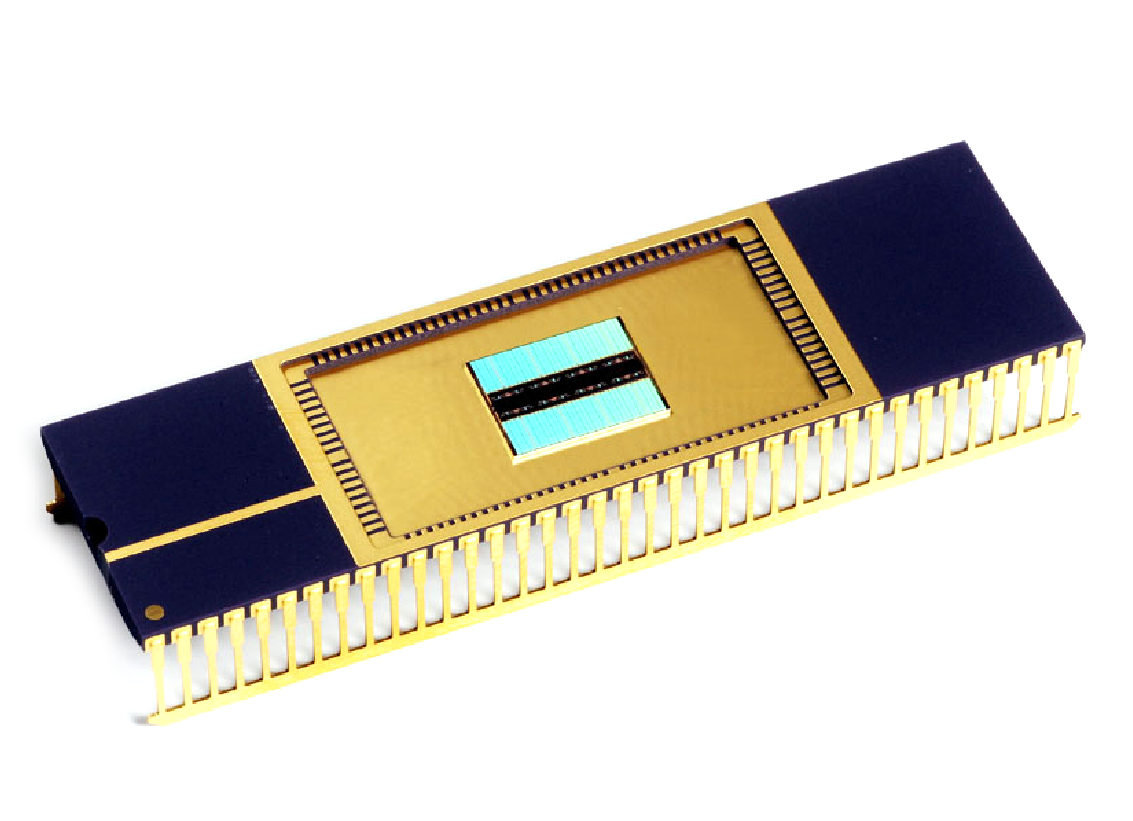
\includegraphics[angle=0, width=0.4\textwidth]{PCM}\\
  \end{minipage}
\end{minipage}
\vspace{1cm}\\
\onslide<2->{
Leghe di calcogenuri: {\ev \gete}, \textcolor{themecolor}{\textbf{\ce{Ge2Sb2Te5} (GST)}}\\[6pt]
%\vspace{0.5cm}
Rapida e reversibile transizione tra cristallo e amorfo ($\sim\SI{50}{ns}$)
}
\end{frame}


\begin{frame}{Materiali a cambiamento di fase}
\begin{table}
\begin{center}
\begin{tabular}{lcl}
Due stati della memoria & \arrowright & bit ``0'' o ``1''\\
\end{tabular}
\vspace{.5cm}\\
%\onslide<2->{
Grande differenza nelle proprietà tra le due fasi \\
%\vspace{1cm}
\begin{tabular}{ccc}
Fase cristallina & {\scriptsize $\arrowright$} & metallica \\
\end{tabular}
\quad
\begin{tabular}{ccc}
Fase amorfa & {\scriptsize $\arrowright$} & isolante\\
\end{tabular}
%}
\vspace{3ex}\\
%\onslide<3->{
\begin{tabular}{lcl}
Variazione di resistività di 3 ordini di grandezza & {\tiny $\arrowright$} & PCM\\
Differenza della riflettività del 30\% & {\tiny $\arrowright$} & memorie ottiche\\
\end{tabular}
\vspace{0.5cm}\\
La transizione è indotta per riscaldamento (impulsi laser/corrente)
%}
\end{center}
\end{table}
\end{frame}


\begin{frame}{Cella PCM}
\begin{columns}
 \begin{column}{0.5\textwidth}
  \begin{itemize}
   \item Regione attiva: piccola porzione del film di materiale a cambiamento di fase che subisce la transizione
   \item Transizione indotta per effetto Joule
  \end{itemize}
 \end{column}
 \begin{column}{0.5\textwidth}
   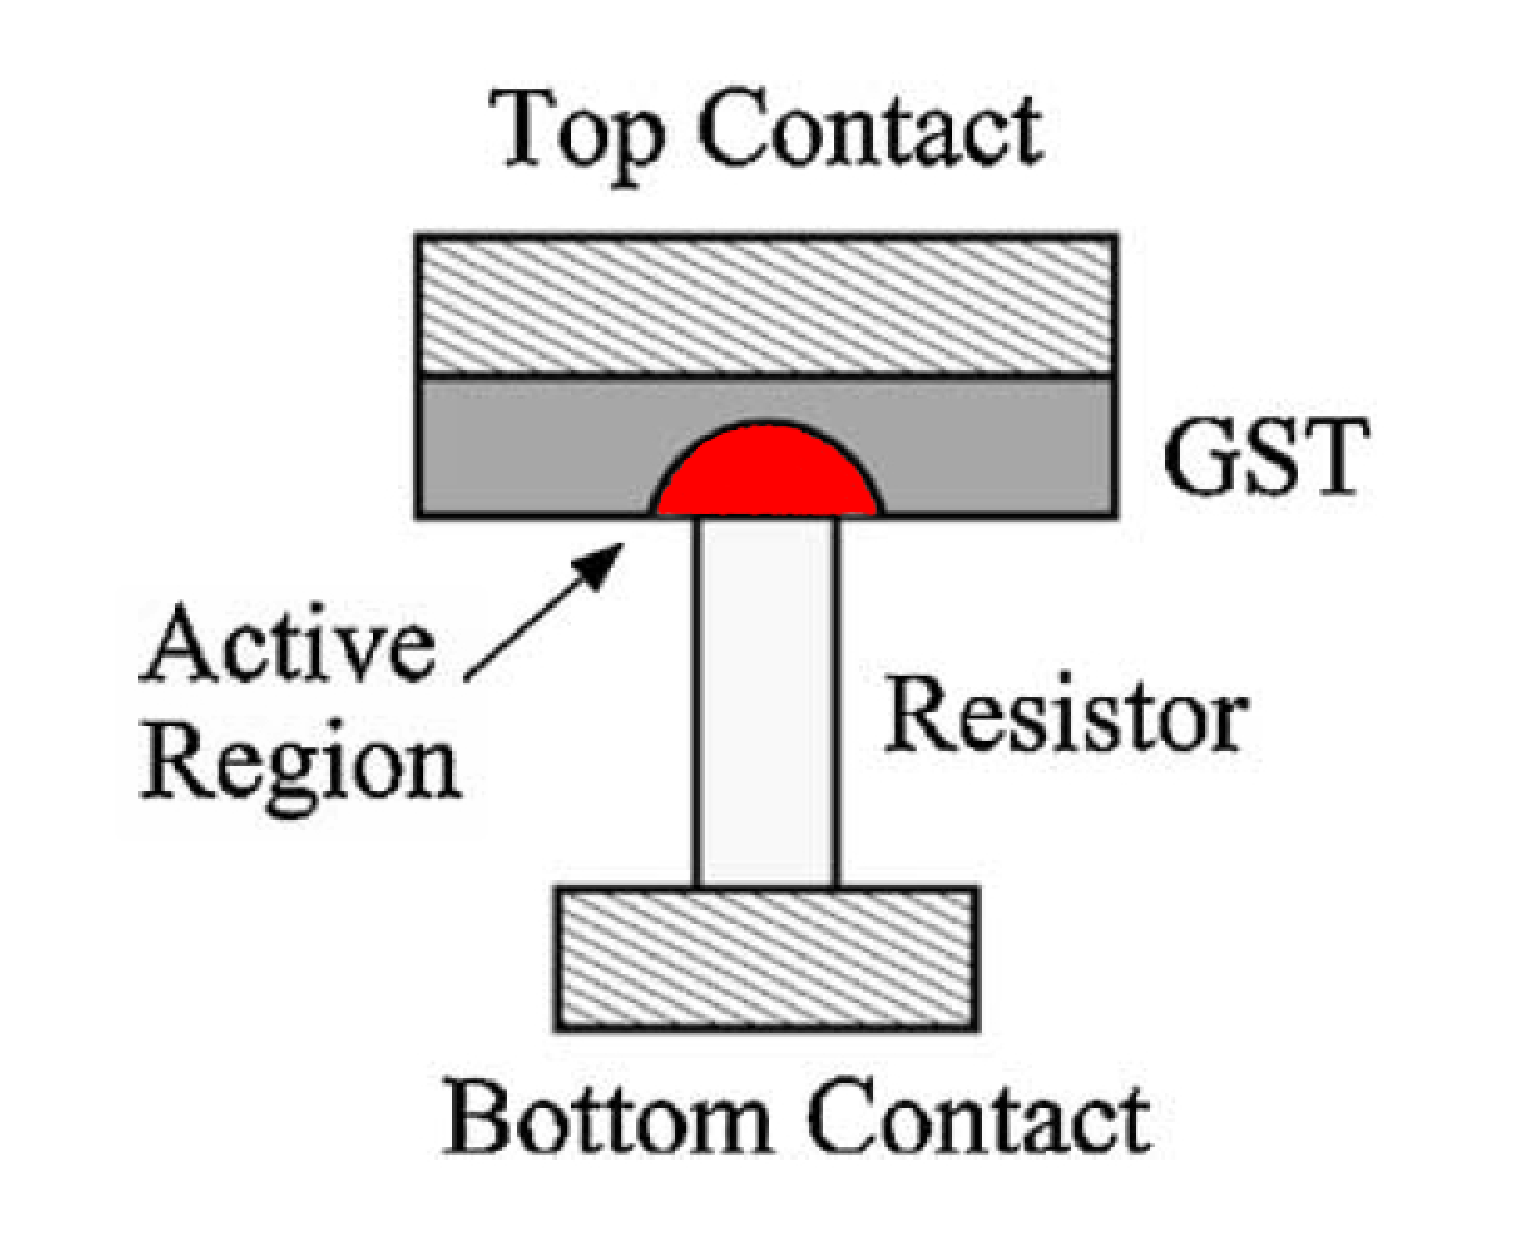
\includegraphics[scale=0.2]{PCMschem}
  %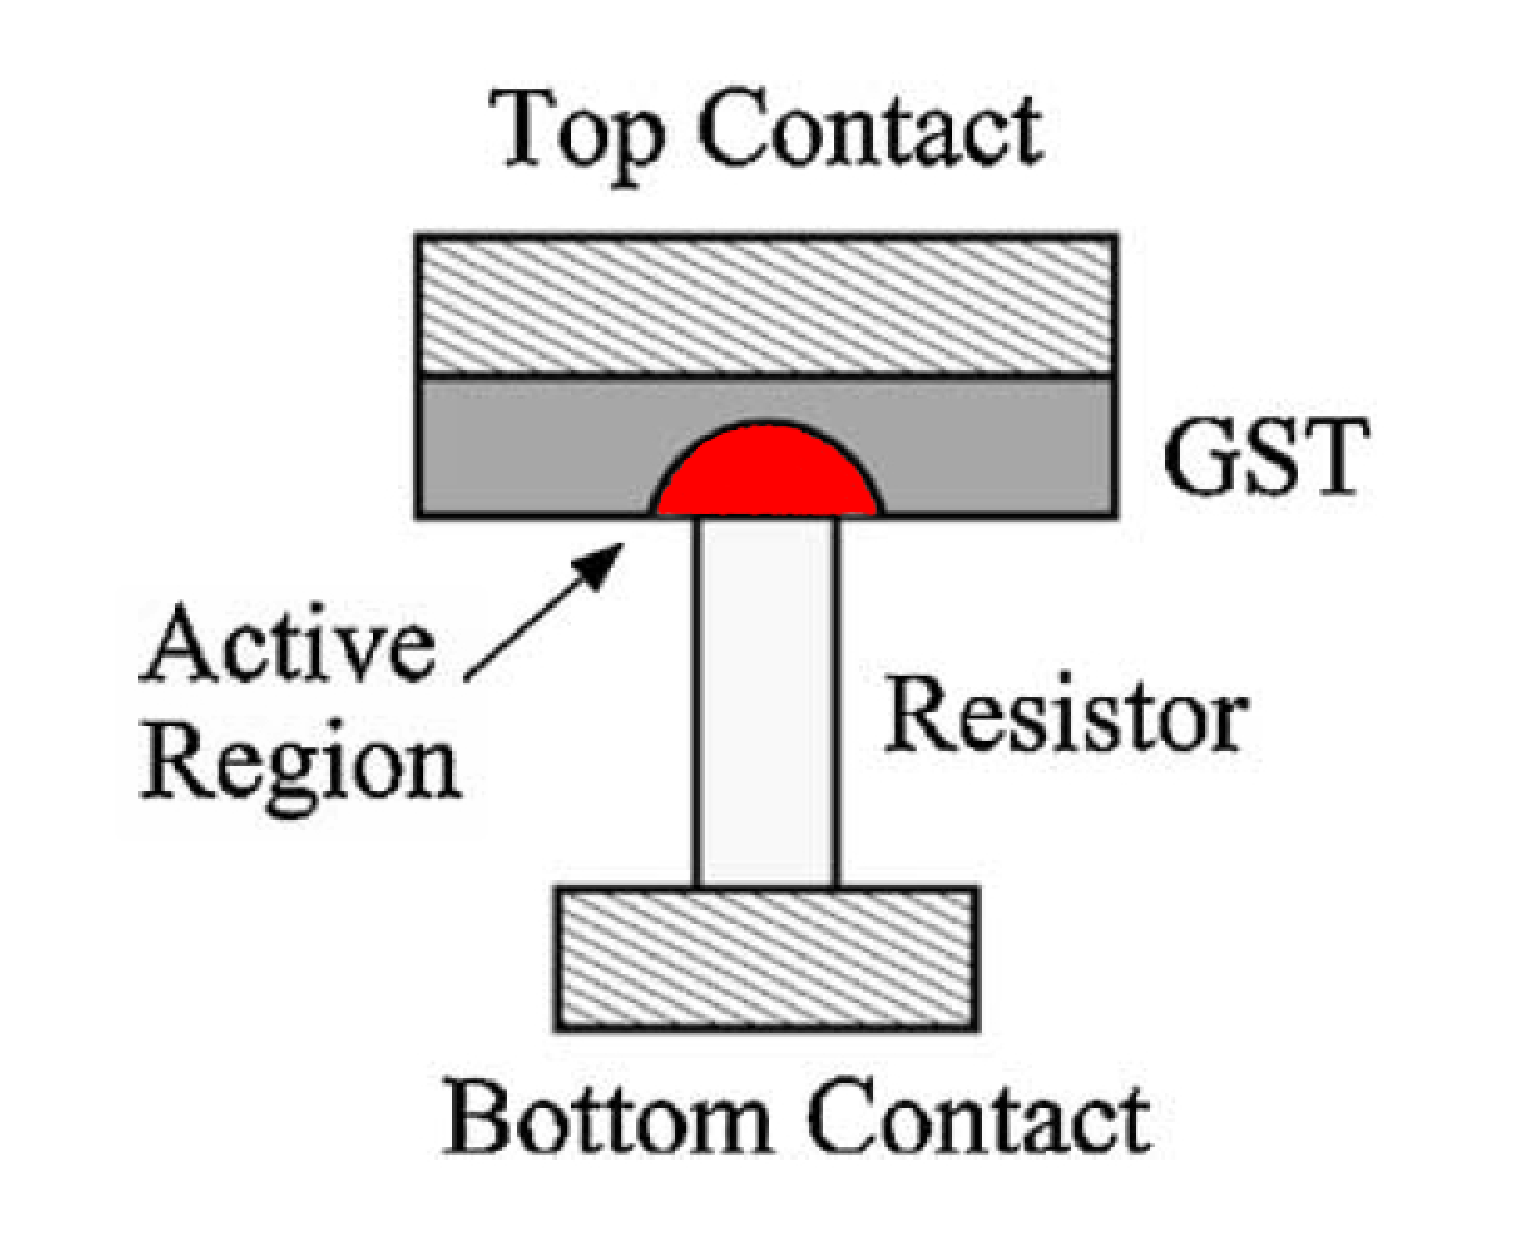
\includegraphics[width=0.5\textwidth]{PCMschem}
 \end{column}
\end{columns}
\end{frame}

%\begin{minipage}[c]{0.58\linewidth}
%\begin{flushright}
%\end{flushright}
%\end{minipage}
%\vspace{-0.05\textheight}
%\begin{minipage}[c]{0.38\linewidth}
%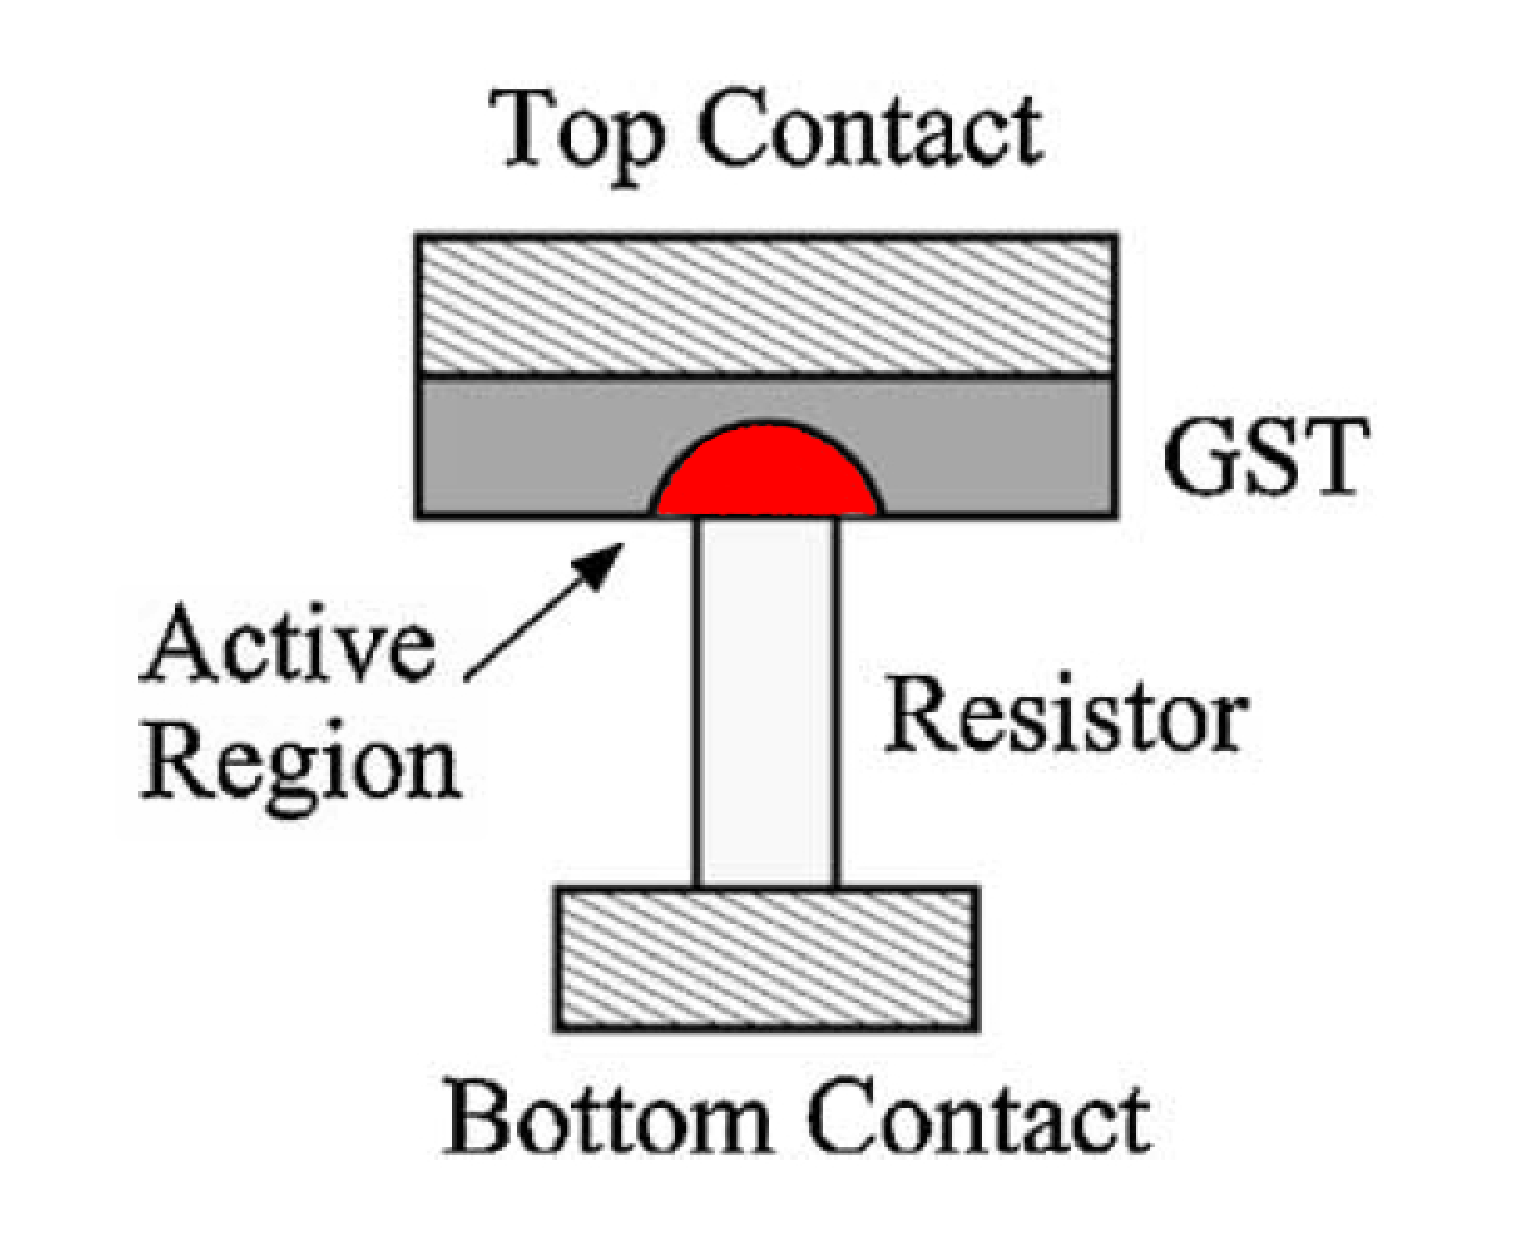
\includegraphics[angle=0, width=0.9\textwidth]{PCMschem.eps}\\
%\end{minipage}
%\begin{minipage}[c]{0.48\linewidth}
%\centering
%\includegraphics[angle=0, width=0.9\textwidth]{PCM_SEM.eps}
%\end{minipage}
%\vspace{2ex}
%\begin{minipage}[c]{0.48\linewidth}
%\small{
%\begin{itemize}
%\item Active region: a small drop within GST film undergoes the phase transition\\
%\item Phase-change by heating via Joule effect
%\end{itemize}
%\begin{center}
%Concept first proposed by\\
%Ovshinsky in 1968
%\end{center}
%}
%\end{minipage}

\begin{frame}{Caratteristica I--V di una cella PCM}
\begin{columns}
 \begin{column}{0.5\textwidth}
  \begin{itemize}
    \item<2-> \emph{Lettura}: eseguita a bassa tensione ($V < V\ped{th}$)
    \item<3-> Processi di \emph{set/reset}: tensione applicata maggiore del valore $V\ped{th}$)
    \begin{itemize}
      \item<3-> \emph{Reset}: elevata intensità di corrente e impulso breve \\
		\ev{cristallo} $\rightarrow$ \ev{amorfo}
      \item<4-> \emph{Set}: bassa intensità e impulso più lungo \\
		\ev{amorfo} $\rightarrow$ \ev{cristallo}
    \end{itemize}
   \end{itemize}
 \end{column}
  \begin{column}{0.5\textwidth}
   \includegraphics<1>[angle=0, width=1.0\textwidth]{IV1}
   \includegraphics<2>[angle=0, width=1.0\textwidth]{IVr}
   \includegraphics<3>[angle=0, width=1.0\textwidth]{IVres}
   \includegraphics<4>[angle=0, width=1.0\textwidth]{IVs}
  \end{column}
\end{columns}
\end{frame}

\begin{frame}{Nanofili nei dispositivi PCM}
 \begin{exampleblock}{Vantaggi nell'utilizzo di nanofili}
  \begin{itemize}
   \item<1-> Riduzione della potenza dissipata nel processo di programmazione
   \item<2-> Riduzione delle dimensioni della cella 
  \end{itemize}
\end{exampleblock}
\note<1>{%
  Sono state proposte diverse architetture per ridurre la potenza dissipata nel processo di programmazione. Una di queste consiste nel sostituire al film di materiale attivo, un nanofilo, che permette un miglior confinamento del calore e in principio consente anche una riduzione delle dimensioni della cella.
}
\end{frame}


\begin{frame}{La cristallizzazione}
 \begin{alertblock}{}
  La cinetica di cristallizzazione è di difficile approccio sperimentale 
 \end{alertblock}

\end{frame}



\section{Nanofili di \gete}

\begin{frame}{Il \gete}
 \begin{columns}
  \begin{column}{0.4\textwidth}
      \begin{itemize}
       \item<1-> Struttura cristallina trigonale (fase $\alpha$): cella elementare romboedrica
       \item<2-> Struttura cubica tipo \ce{NaCl} elongata lungo la $\langle 111 \rangle$
       \item<3-> Parametri strutturali
      \onslide<3->{% 
       \begin{itemize}
        \item $a=\SI{4.31}{\angstrom}$
        \item $\alpha=\ang{57.9}$
        \item $x=\num{0.2366}$ \\[3pt] Ge: $(x,\,x,\,x)$ \\[3pt] Te: $(-x,\,-x,\,-x)$
       \end{itemize}}
       \note<3>{%
	 I parametri strutturali della struttura trigonale sono il passo reticolare $a$, l'angolo tra una coppia di vettori di base $\alpha$ e il parametro $x$ che assegna le posizioni nella cella elementare dei due atomi di Ge e Te. 
	}
      \end{itemize}
  \end{column}
  \begin{column}{0.4\textwidth}
   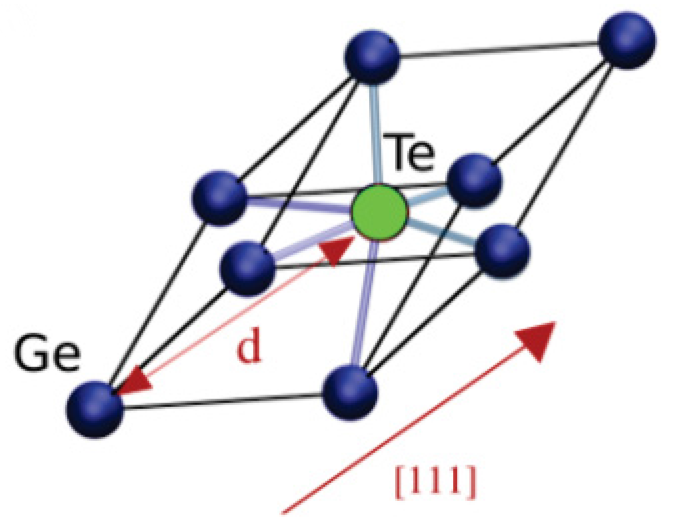
\includegraphics[width=0.7\textwidth]{GeTe-cell}\\[12pt]
   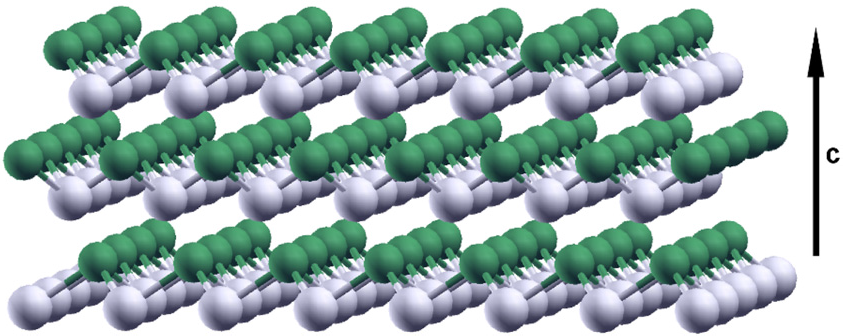
\includegraphics[width=\textwidth]{GeTe-bilayer}
  \end{column}

 \end{columns}

\end{frame}

\begin{frame}{Nanofili: il modello}
 Nanofili: il modello
\end{frame}





\section{Metodi computazionali}
%\subsection{Potenziale \emph{neural networks}}
\begin{frame}{Dinamica molecolare con potenziale \emph{neural networks}}
 MD e potenziale NN
\end{frame}

\begin{frame}{Potenziale \emph{neural networks}}
 \centering
Total energy as a sum of the atomic energies: $E_{tot} = \sum_i E_i$
\begin{flushright}
{\cit{[Behler J. and Parrinello M., Phys. Rev. Lett. 2007]}}
\end{flushright}
\vspace{3ex}
\begin{columns}[c]
\column{0.50\textwidth}
\begin{displaymath}
E_i = F(\{G(\bar{x})\}) 
\end{displaymath}
\column{0.50\textwidth}
\centering
{\ev{Symmetry functions $\{G\}$}}\\
Information on the atomic environment
up to a certain cut-off radius
(3$^{rd}$ coordination shell)\\
\end{columns}
\vspace{2ex}
\begin{columns}[c]
\column{0.50\textwidth}
\centering
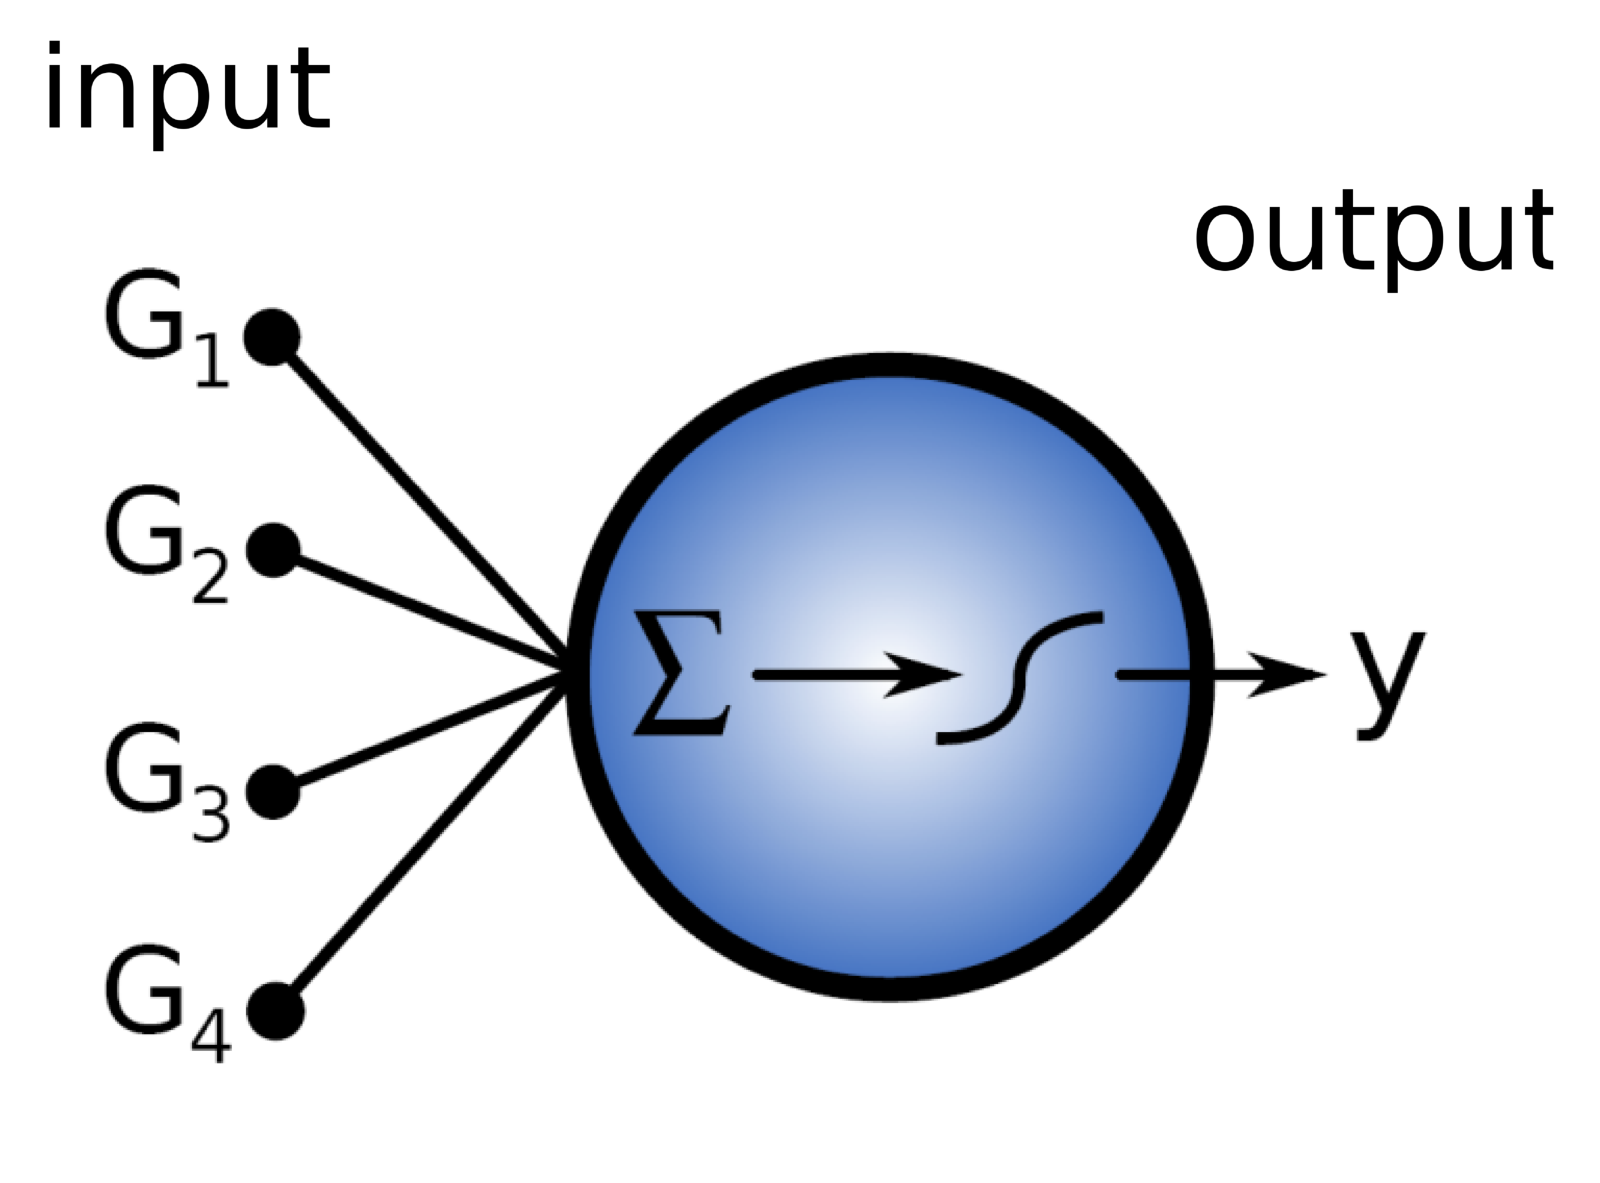
\includegraphics[angle=0, width=0.7\textwidth]{NN_schema}
\column{0.50\textwidth}
$E_i$ analytic function of the atomic positions
\end{columns}
\end{frame}




%\section{Risultati}


\end{document}


